\documentclass{article}
\usepackage{longtable}
\usepackage{xcolor}
\usepackage{enumitem}
\usepackage{geometry}
\usepackage{float}
\usepackage{url}
\usepackage{graphicx}
\usepackage{amsmath}
\usepackage{listings}
\usepackage{microtype
}

\newcommand\ytl[2]{
    \parbox[b]{12em}{\hfill{\color{cyan}\bfseries\sffamily #1}~$\cdots\cdots$~}\makebox[0pt][c]{$\bullet$}\vrule\quad
    \parbox[c]{10cm}{\vspace{6pt}\color[RGB]{20, 20, 90}\raggedright\sffamily #2\par}
    \\[-2pt]
}





\title{Creating Software for Value at Risk}
\author{Benjamin Shearlock}

\begin{document}
\raggedright

\begin{titlepage}
  \begin{center}
    \vspace*{1cm}
    {\LARGE \textbf{Creating Software for Value at Risk} \par} 
    \vspace{1.5cm}
    {\Large \textit{Interim Report} \par}
    \vspace{0.5cm}
    {\Large BSc Final Year Project \par}
    \vspace{2cm}
    {\large \textbf{Author} \par}
    {\large Benjamin Shearlock \par}
    \vspace{2cm}
    {\large \textbf{Supervisor} \par}
    {\large Dr. Volodya Vovk \par}
    \vfill
    {\large Department of Computer Science \par}
    {\large Royal Holloway, University of London \par}
  \end{center}
\end{titlepage}

\setlength{\parindent}{0pt}

\section*{Declaration}
I have read and understood the Universities regulations on plagiarism and I hereby declare that all work submitted in this project is my own, except where explicitly stated otherwise, such as the references that have been cited. \\

\begin{itemize}
  \item Word Count: 0
  \item Name: Benjamin Charles Shearlock
  \item Submission Date: 08/12/2023
  % \item Signature: \includegraphics[scale=0.1]{Signature.png}
\end{itemize}

\newpage

\tableofcontents

\newpage

\section{Abstract}
In the realm of financial risk management, understanding and evaluating the level of risk associated with any investment or portfolio is of extremely high importance. Perhaps the most universally regarded metric used for this purpose is Value at Risk (VaR). VaR provides a quantitative estimate of the potential losses that a portfolio may incur over a certain period of time (specified time horizon) at a given confidence level. \\\vspace{0.3cm}

Original widespread use of VaR came about in the early 1990s, the concept first being introduced by J.P. Morgan in 1994, since it helped provide an estimate of the maximum loss an investor is willing to accept for any given investment. Its historical roots can be traced back to the financial industry's increasing need for a standardized and comprehensive measure of risk following the 1987 stock market crash, so they sought a comprehensive way to assess risk in complex portfolios [\ref{ref3}]. \\

Mathematically, VaR is expressed as follows:
\begin{equation}
VaR(N, X) = -\text{Percentile}(L, 1 - X)
\end{equation}
Where:
\begin{align*}
N & : \text{Time horizon (in days)} \\
X & : \text{Confidence level (in percentage)} \\
L & : \text{Loss distribution over } N \text{ days}
\end{align*}

This formula captures the loss at the \((100-X)\)th percentile of the loss distribution over the specified time horizon [\ref{ref6}]. \\\vspace{0.3cm}

VaR can be mathematically computed through various methods, each with its own strengths and limitations. The most common approaches include the historical simulation method, parametric method, model building method and Monte Carlo simulation [\ref{ref1}], to list a few. For historical simulation, past data is used to estimate future risk by examining the historical returns of an asset or portfolio, while model building employs mathematical models to predict portfolio performance. The choice of algorithm depends on data availability, computational resources, and specific requirements.\\\vspace{0.3cm}

To implement VaR calculations, various pieces of software are essential. In this project, I will be utilising Visual Studio Code (VSCode) as the integrated development environment (IDE) and Python for its rich ecosystem of libraries. Python libraries like NumPy, Matplotlib, and Kivy will be invaluable for data manipulation, visualisation, and user interface design [\ref{ref9}].\\\vspace{0.3cm}

My inaugural proof of concept program will be created to visually demonstrate VaR calculations for  two initial methods, these being historical simulation and model building techniques to estimate VaR for a sample portfolio. Historical simulation would involve collecting historical data and computing VaR based on past performance (can involve acquiring stock data through an API), while model building would use a predefined model to forecast future losses. Visualisation tools like Matplotlib can help in presenting the results graphically, enabling me to generate informative charts and graphs. NumPy will facilitate data manipulation and efficient mathematical operations [\ref{ref10}]. Additionally, Kivy, a Python framework for developing multi-touch applications, will be used to create the interfaces for the visual representation of VaR, as well as giving it the option to possibly be viewed on other devices.\\\vspace{0.3cm}

Later on into the project, if there is enough time, I think it may be worth exploring some more advanced topics like the variance-covariance of returns, specifically employing GARCH (Generalized Autoregressive Conditional Heteroscedasticity) models. GARCH models provide a more nuanced understanding of volatility and can enhance the accuracy of VaR estimates [\ref{ref6}].\\\vspace{0.3cm}

The objective of my project is to gain a deeper understanding of VaR, develop a functional program to calculate and visualise it, and potentially extend the research to incorporate more advanced risk management techniques if possible. This project is a stepping stone towards a deeper understanding of the risk side of finances and will contribute to enhancing the knowledge and skills necessary for effective financial decision-making, since this is not a topic that I have delved much into before, but I have aways been very interested in learning more about it. This gives me a fantastic opportunity to learn about the financial sector, as well as create something that is applicable and useful to real life. \\


% \section{Specification}

\newpage
\section{Chapter 1 - Introduction}

\subsection{What is VaR?}

Value at Risk (VaR) is a statistical value used to quantify the level of financial risk within a portfolio of stocks/derivatives over a specified time horizon. It estimates the maximum potential loss that an investment portfolio could incur with a given probability, known as the confidence level, under normal market conditions. The VaR metric is typically expressed in monetary terms and is often used to assess the risk of a portfolio of financial instruments. From a banks perspective, they would say:
\begin{quote}
  ``With \textbf{X\% confidence (1-X\% Risk Level)}, we expect to not lose more than \textbf{V} over the next \textbf{N day(s)} on our entire \textbf{portfolio} of derivatives, worth \textbf{Z}'' %[\ref{ref4}]

\end{quote}

Where:
\begin{align*}
  \textbf{X} & : \text{Confidence Level} \\
  \textbf{V} & : \text{Value at Risk} \\
  \textbf{N} & : \text{Time Horizon} \\
  \textbf{Z} & : \text{Portfolio Value}
\end{align*}

This is incredibly useful as it allows for a simple and easy to understand metric to be used to assess the risk of a portfolio, which is extremely important in the financial sector, taking all the underlying complexities of any form of portfolio and being able to conform its financial risk into a single, universally used, number. \\\vspace{0.3cm}

To include actual numbers, to easier explain how it would look, a bank would say:
\begin{quote}
  ``With \textbf{95\%} confidence (\textbf{5\%} Risk Level), we expect to not lose more than \textbf{£3,000,000} over the next \textbf{1 day} on our entire portfolio of derivatives, worth \textbf{£100,000,000}''
\end{quote}

This is essential to help financial institutions understand the level of risk associated with their portfolios, as well as being able to compare the risk of different portfolios, which is why it is such a widely used metric in the financial sector, limiting the level of risk that a person/organisation is exposed to.\\\vspace{0.3cm}

The concept of VaR has its roots in the late 20th century, gaining prominence in the finance industry during the 1990s. It emerged from the need for more sophisticated risk management tools in the wake of financial market liberalisation and the increasing complexity of financial instruments. The widespread adoption of VaR was catalysed by the 1998 financial crisis, where it played a significant role in risk assessment and regulatory frameworks.\\\vspace{0.3cm}


VaR is significant for several reasons:
\begin{itemize}
    \item \textbf{Risk Measurement:} VaR provides a quantitative measure of potential losses in a portfolio.
    \item \textbf{Decision Making:} VaR aids financial managers in making informed decisions about risk tolerance and capital allocation.
    \item \textbf{Market Risk Management:} VaR is used to monitor and mitigate market risks, contributing to the overall stability of financial systems.
\end{itemize}

VaR has become a cornerstone in risk management for global financial markets. It is used by banks, investment firms, asset managers, and corporates to measure and control the level of risk exposure in their financial portfolios. VaR's adoption is partly driven by regulatory requirements, such as Basel Accords, which mandate financial institutions to calculate and maintain adequate capital reserves based on their risk exposure.\\\vspace{0.3cm}


Developing software for VaR calculation offers numerous advantages:
\begin{itemize}
    \item \textbf{Accessibility:} It democratizes the access to sophisticated risk management tools.
    \item \textbf{Efficiency:} Automated VaR calculations save time and reduce the potential for human error.
    \item \textbf{Customization:} Software can be tailored to specific needs and types of portfolios.
    \item \textbf{Real-Time Analysis:} It enables rapid and up-to-date risk assessments.
\end{itemize}

VaR has become an essential tool in modern financial risk management. The development of software for VaR calculations aligns with the need for efficient, accurate, and accessible risk management tools in today's fast-paced financial markets. This is what I want to help contribute to within this project.\\

\subsection{Aims and Goals}
My aims and goals for this project are as follows:

\begin{enumerate}
    \item \textbf{Comprehensive Understanding of VaR:} To touch on VaR's theoretical underpinnings and why it has such a pivotal role in modern financial risk management. This includes commenting on its applications across different financial groups, market conditions, and regulatory environments.
    
    \item \textbf{Methodological Exploration:} To investigate various computational methods for calculating VaR, including historical simulation, model building (variance-covariance) approach, and Monte Carlo Simulation, assessing their efficacy in different market scenarios. This will first be explored through command line programs, then later on through a GUI\@.
    
    \item \textbf{Technical Implementation:} Development of a comprehensive program for calculating and presenting VaR. This entails creating a user-friendly interface, ensuring accurate and efficient computation, and integrating various methods of VaR calculation to provide a comprehensive tool.
    
    \item \textbf{Application in Diverse Financial Contexts:} To ensure the software's adaptability and applicability in different financial settings. This includes testing the software with various data sets, portfolio types, and market conditions, aiming to make it a versatile tool for different financial entities.
    
    \item \textbf{Industry Standard Tool Development:} Creating a software application that not only performs standard VaR calculations but also offers other stock-oriented features, such as advanced data visualization. The goal is to make the tool align with industry standards, ensuring it is suitable for professional financial risk management and has been developed whilst adhering to to industry principles in regard to software engineering.
\end{enumerate}

The ambition of this thesis is to present a thorough understanding of VaR, culminating in the development of a robust, adaptable, and industry-relevant tool for financial risk assessment. It aims to be acceptable as an industry standard tool, 
  
\subsection{Milestone Plan}
Due to unfortunate circumstances, I had rough delays to the start of this Project as well as inconsistent health concerns, but that should not effect my overall final deliverable. In the first term, I want to research and create a working program to compute Value at Risk for small portfolios, that has a serviceable GUI that can be expanded on later. I will also make sure to have amply researched about back-testing and how to incorporate it into my program in some capacity. For the second term, I will research and implement applying Value at Risk for a portfolio of derivatives, as well as looking into using the Monte Carlo simulation and allowing for the computation of all this with as many stocks as necessary. I will finalise the GUI and plan to look into completing some of the extensions provided for the project, this will depend on the overall developmental scope of the project at the time, but these are the options I would be willing to explore:

\begin{itemize}
  \item \textbf{Computing Conditional VaR (Expected Shortfall):}  Beyond the standard VaR metric, exploring Conditional VaR could be considered to provide a more comprehensive risk assessment, as it accounts for the severity of losses in the tail of the distribution.

  \item \textbf{Parameter Selection for EWMA and GARCH(1,1) Models:} A detailed analysis of parameter selection for the Exponentially Weighted Moving Average and GARCH(1,1) models could be explored. The choice of parameters greatly influences model performance, and overall it would enhance the robustness of the risk assessment.
  
  \item \textbf{Empirical Study of Approaches to Historical Simulation for n-day VaR:} A comparative empirical study could be undertaken to examine different approaches to extending historical simulation from 1-day to n-day VaR, which can provide deeper insights into the performance of the methods.
  
  \item \textbf{Complementing Back-Testing by Stress Testing:} The robustness of the VaR model could be assessed not only through back-testing but also by applying stress testing techniques, allowing for the evaluation of the model's performance under extreme market conditions.
  
  \item \textbf{Computing Monetary Measures of Risk Different from VaR:} Other monetary risk metrics, which could complement or provide alternatives to VaR, such as Tail Value at Risk, could be considered to present a more complete picture of the risk landscape and enhance the risk management process.
\end{itemize}

The project's milestones have been structured to ensure a systematic and efficient approach to the development of the Value at Risk software. This plan is divided into distinct phases, each with specific objectives and deliverables.

  \begin{enumerate}
    \item \textbf{Initial Research and Planning (Completed):} This phase involved a thorough investigation into the concept of Value at Risk, its calculation methods, and the requirements for the software development.
    \item \textbf{Software Design and Development (Ongoing):} Currently, the focus is on designing the software and developing the core functionalities of the VaR calculation tool. This includes building the initial graphical user interface and implementing various VaR models into it.
    \item \textbf{Expanded GUI, Testing and Refinement:} After the development phase, there will be a complete redesign/refinement of the Graphical Interface, followed by rigorous testing that will be conducted to ensure the accuracy and reliability of the software. This phase will also involve refining the user interface and the overall user experience.
    \item \textbf{Final Evaluation and Documentation:} The final phase involves a comprehensive evaluation of the software against the project's objectives and preparing detailed documentation as well as informational videos.
  \end{enumerate}

  \subsubsection{Timescale}
  The entire project is structured over two academic terms, allowing ample time for each phase while ensuring a steady progression towards the project's completion. This timescale is designed to balance the initial development and subsequent refinement and testing phases effectively, ensuring that each aspect of the software is given due attention.\\\vspace{0.3cm}

  Concurrent with the development, ongoing documentation is a critical aspect of this project. Documenting the process as it unfolds serves multiple purposes: it ensures a clear record of the development process and aids in identifying and resolving issues more efficiently. This approach to documentation not only enhances the quality and maintainability of the software but also ensures that the project's progress is well-documented and aligns with the overall objectives and milestones.

  \subsubsection{Timeline}
\vspace{-2\baselineskip}
\begin{table}[H]
  \centering
  \color{black}
  \begin{longtable}{p{1\linewidth}}
    \endfirsthead
    \endhead
    \hspace*{\dimexpr\linewidth-0.721\linewidth}\rule{0.7\linewidth}{0.4pt}
    \ytl{Weeks 1--3}{
      \textbf{Project Research}
      \vspace{8pt}
      \begin{itemize}
          \item Research the fundamentals of Value at Risk (VaR)
          \item Research best coding language to use (Python)
          \item Familiarize myself with LaTeX and prepare IDE \& Git for Project specified use
      \end{itemize}
    } \vskip-19pt\hspace*{\dimexpr\linewidth-0.721\linewidth}\rule{0.7\linewidth}{0.4pt}
    \ytl{Week 4}{
      \textbf{Finalize Plan and Start Coding}
      \begin{itemize}
          \item Complete Project Plan
          \item Continue researching VaR and Python
          \item Begin project coding
      \end{itemize}
    } \vskip-19pt\hspace*{\dimexpr\linewidth-0.721\linewidth}\rule{0.7\linewidth}{0.4pt}
    \ytl{Week 5--7}{
      \textbf{Coding and Data Preparation}      
      \begin{itemize}
          \item Continue to work on the VaR program (No GUI)
          \item Start collecting and organizing sample data for small portfolios so it can be used by the program
          \item Finalizing understanding of the two computational methods needed, this being model-building and historical simulation
      \end{itemize}
    } \vskip-19pt\hspace*{\dimexpr\linewidth-0.721\linewidth}\rule{0.7\linewidth}{0.4pt}
    \ytl{Week 8}{
      \textbf{Back-Testing Research \& Implementation}      
      \begin{itemize}
          \item Investigate methods and techniques for VaR back-testing
          \item Start integrating back-testing into the project
      \end{itemize}
    } \vskip-19pt\hspace*{\dimexpr\linewidth-0.721\linewidth}\rule{0.7\linewidth}{0.4pt}
    \ytl{Week 9--10}{
      \textbf{GUI Development}      
      \begin{itemize}
          \item Initiate the development of the GUI
          \item Ensure the GUI is robust for its current task as well as expandable for future enhancements
      \end{itemize}
    } \vskip-19pt\hspace*{\dimexpr\linewidth-0.721\linewidth}\rule{0.7\linewidth}{0.4pt}
    \ytl{Week 11}{
      \textbf{Interim Report and Presentation Preparation}      
      \begin{itemize}
          \item Fine-tune programs and report so they are at a satisfactory level, will also allow for easier preparation for the interim presentation 
          \item Prepare for the interim presentation 
      \end{itemize}
    } \vskip-19pt\hspace*{\dimexpr\linewidth-0.721\linewidth}\rule{0.7\linewidth}{0.4pt}
  \end{longtable}
\end{table}

\vspace{-2\baselineskip}
\begin{table}[H]
  \centering
  \color{black}
  \begin{longtable}{p{1\linewidth}}
    \endfirsthead
    \endhead
    \vskip-19pt\hspace*{\dimexpr\linewidth-0.721\linewidth}\rule{0.7\linewidth}{0.4pt}
    \ytl{Weeks 1--2}{
      \textbf{Reflection and Research}
      \vspace{8pt}
      \begin{itemize}
          \item Spend time to reflect on the progress of the project so far, make any changes that I think are warranted after having the winter break time to think about
          \item Research the Monte Carlo simulation method for VaR, as well as how I could start implementing derivatives as portfolios into the project
      \end{itemize}
    } \vskip-19pt\hspace*{\dimexpr\linewidth-0.721\linewidth}\rule{0.7\linewidth}{0.4pt} 
    \ytl{Week 3--4}{
      \textbf{Start Implementing New Features}
  
      \begin{itemize}
          \item Start implementing the Monte Carlo simulation method and continue derivative implementation
          \item Start researching Eigen \& Cholesky decomposition to allow for however many stocks are needed within a portfolio
      \end{itemize}
    } \vskip-19pt\hspace*{\dimexpr\linewidth-0.721\linewidth}\rule{0.7\linewidth}{0.4pt} 
    \ytl{Week 5--7}{
      \textbf{GUI Finalisation}
      \begin{itemize}
          \item Decide on the final visual product I want to represent with the GUI and start implementing it (if progress on this needs to continue into the next period, then it will be done so)
          \item Set the program up to work portably/allowing it to work on mobile OS's as well as different desktop OS's
      \end{itemize}
    } \vskip-19pt\hspace*{\dimexpr\linewidth-0.721\linewidth}\rule{0.7\linewidth}{0.4pt} 
    \ytl{Week 8--9}{
      \textbf{Extend Project Scope (if time permits)}
      \begin{itemize}
          \item Explore additional features or enhancements for the project, possibly decided upon at the start of Term 2
          \item Implement as many as can be appropriately managed, with all additional time spent within this period being used to ensure the project is at its most refined state
      \end{itemize}
    } \vskip-19pt\hspace*{\dimexpr\linewidth-0.721\linewidth}\rule{0.7\linewidth}{0.4pt} 
    \ytl{Week 10--11}{
      \textbf{Perfect Final Report}
      \begin{itemize}
          \item Make sure the program has been achieved to the best of its ability
          \item Finalise and perfect the final report
      \end{itemize}
    } \vskip-19pt\hspace*{\dimexpr\linewidth-0.721\linewidth}\rule{0.7\linewidth}{0.4pt} 
  \end{longtable}
\end{table}

\newpage

\section{Chapter 2 --- Understanding VaR}

\subsection{Historical Simulation}

Historical Simulation is a method of estimating Value at Risk (VaR). It relies on historical market data to predict future risks, making it a straightforward yet powerful method for calculating VaR. The process of computing VaR through Historical Simulation involves several steps, as outlined below:

\begin{enumerate}
    \item \textbf{Data Collection:} Historical price data of the asset is collected for a specified time period. This can be done using an API or through a CSV file.
    \item \textbf{Calculate Percentage Differences:} The daily returns are calculated, this being done by comparing the closing price of the current day to the closing price of the previous day by dividing one by the other, the taking away 1. This is done for each day in the data set.
    \item \textbf{Sort Returns:} The calculated returns are sorted in ascending order.
    \item \textbf{Determine the VaR Threshold:} A percentile is chosen based on the confidence level (e.g. 95\%). This is used to work out 100\% - X percentile (e.g. 5th), this being the risk level of the portfolio and X being the confidence level. This is the VaR threshold.
    \item \textbf{VaR Estimation:} The Value at Risk is estimated as the value at the chosen percentile. For example, if you have 500 days of data, the 5th percentile would be the 25th value in the sorted list of returns, then multiplied by the portfolio value, simulating the worst percentage decrease that your portfolio could encounter based on the last Z days of data.
    \item \textbf{Correct Negative Number:} Since it takes the 5th percentile, it will be a negative percentage difference multiplied by the portfolio, since we need to represent VaR as a positive value of potential loss, it is multiplied by -1 to make it positive.
\end{enumerate}

As you can see, it takes a very literal approach, assuming that, since you've got all this historical data, then it is likely that the future will be similar to the data of the past. It is an empirical method, meaning it is based on historical data, and as such is a simple and easy to understand, but it does have its limitations, such as the fact that it does not take into account any changes in the market, such as a financial crisis, which could have a huge impact on the market.\\\vspace{0.3cm}

\begin{figure}[h]
  \centering
  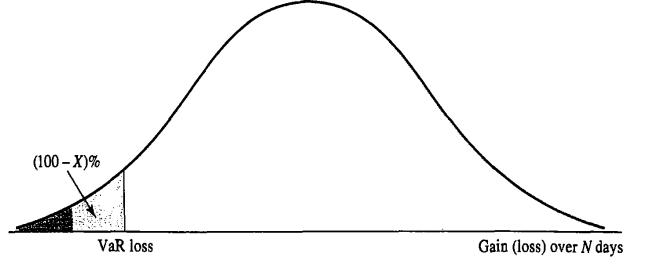
\includegraphics[width=0.5\textwidth]{Images/Image 1.png}
  \caption{The Value at Risk (VaR) is calculated from the probability distribution of the variations in the portfolio's value, where gains are represented as positive values and losses as negative. The confidence level for this calculation is set at X\%. [\ref{ref4}]}
  \label{VaR Distribution Curve}
\end{figure}

Refer to Figure~\ref{VaR Distribution Curve}, it expresses that:  
\begin{itemize}
  \item The bell-shaped curve represents the probability distribution of gains and losses for the asset or portfolio over the specified period.
  
  \item The left tail of the distribution marks the area of losses, where we can observe the VaR loss at a specific confidence level, say \( (100 - X)\% \). This tail area signifies the worst losses incurred in the historical period.
  
  \item The point where the left tail cuts the horizontal axis (gain/loss over N days) corresponds to the VaR at the chosen confidence level. For example, if \( X \) is 95, then the VaR would represent the maximum expected loss over the N days period that only 5\% of the time is expected to be exceeded.
  
  \item The graph assumes that the past can be a predictor of future risk, thus the frequency and magnitude of historical losses are directly used to estimate the VaR.
\end{itemize}

\subsection{Model Building (Variance-Covariance)}

The Variance-Covariance method, used in this analysis for Value at Risk (VaR) calculation, is based on the assumption of normally distributed market returns. The key steps in the model are as follows:

\begin{enumerate}
    \item \textbf{Data Collection:} Historical price data of the asset is collected for a specified time period once again. This can be done using an API or through a CSV file.
    \item \textbf{Calculate Daily Returns:} Daily returns are computed as the percentage change in the adjusted closing prices of the stock.
    \item \textbf{Statistical Analysis:} The mean and standard deviation of the daily returns are calculated to represent the average return and the volatility of the stock, respectively.
    \item \textbf{VaR Calculation:} The Value at Risk is calculated using the formula:
    \begin{equation}
      VaR = - P \times (\text{norm.ppf}(rl, \text{mean}, \text{sD}) + 1) 
    \end{equation}
    where:
\begin{itemize}
    \item \( P \) represents the total value of the portfolio.
    \item \( \text{norm.ppf} \) is a function from the \texttt{scipy.stats} library that calculates the inverse of the cumulative distribution function (CDF) of the normal distribution, also known as the Percent Point Function (PPF).
    \item \( rl \) is the risk level, which corresponds to the confidence level for VaR. For example, a 95\% confidence level would use an \( rl \) of 0.05 (5\% risk level).
    \item \( \text{mean} \) and \( \text{sD} \) are the mean and standard deviation of the historical returns, respectively.
\end{itemize}
\end{enumerate}

The Value at Risk (VaR) calculation in the Variance-Covariance method is executed using a specific equation that combines statistical measures with the portfolio value to estimate the potential loss over a specified time horizon. The equation is as follows:

\begin{enumerate}
    \item The \(\text{norm.ppf}\) function takes the risk level \( rl \), mean, and standard deviation of returns as inputs and outputs a Z-score. This score corresponds to the point on the normal distribution curve where the cumulative probability is equal to the risk level.
    \item The equation then multiplies this score with the portfolio value \( P \) and subtracts from \( P \). This represents the potential loss in value of the portfolio at the given confidence level.
    \item The addition of 1 in the formula adjusts for the fact that the \(\text{norm.ppf}\) function returns a negative value for typical VaR confidence levels. This is because the function calculates the Z-score for the left tail of the distribution, while VaR is the loss at the right tail. The addition of 1 converts the negative value to a positive one.
\end{enumerate}

Thus, the equation calculates the VaR as the maximum expected loss over a certain period, given normal market conditions and a specified confidence level. The Variance-Covariance method is a simple yet effective approach to VaR calculation, but it does have its limitations, such as the fact that it assumes that the returns are normally distributed, which is not always the case.\\\vspace{0.3cm}


% \\\vspace{0.3cm}


\subsection{Coding VaR Methods}
To validate that I could apply the knowledge I had gained from my research, I decided to code the two methods of VaR calculation that I had researched, this being the historical simulation and model building methods. I have decided to use Python (3.11.1) as my coding language, as it is a language that I am familiar with and has a rich ecosystem of libraries that I can use to help me with the project. I also decided to use command line to display the results, as it utilises pythons inbuilt \(\text{print()}\) command to easily display variables, allowing for a quick and easy way to display the results of the VaR calculations, as well as any tests run as well. %I have also decided to use yahoo finance as my data source, as it is a free and easy to use API that allows for the collection of historical stock data, which is exactly what I need for this project. 
\\\vspace{0.3cm}

\subsubsection{Command Line --- Historical Simulation}

You code them, here's some code:
\begin{verbatim}
  closes = np.array([])
  with open('NKE.csv', 'r') as file:
      reader = csv.reader(file)
      for row in reader:
          closes = np.append(closes, float(row[5]))
  \end{verbatim}

  \begin{verbatim}
    diffs = np.array([])
    for i in range(1, len(closes)): 
        diffs = np.append(diffs, (closes[i]/closes[i-1] - 1))
    print("500 Day stock history, for 1 day time horizon, 95% certainty, 
    Portfolio of 100,000,000, VaR for the 23/10/2023: £" + 
    str(round(np.percentile(diffs, 5)*100000000*-1, 3)))
    \end{verbatim}

  \begin{figure}[h]
    \centering
    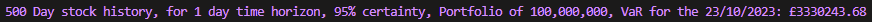
\includegraphics[width=1.1\textwidth]{Images/Historical Command Line Result.png}
    \caption{Your caption}
    \label{fig:your_label}
  \end{figure}

  \subsubsection{Command Line --- Model Building}



\subsection{Back Testing}
I was rather smart with this, including a diagram would be cool but idk how to do that in latex

\subsection{Combining Implementations}
Show how I made the command line program, idk just show off the code and results

\subsection{Multiple Stocks}
Show that I used  some fucking thing that I got from some fucking reference


\section{Chapter 3 - Graphical User Interface}

\subsection{What is Kivy?}

\subsection{Conceptualisation of Initial Design Ideas}
Show my super cool picture I drew and talk about what I want 
\subsection{Initial GUI Creation}
show off stages of the creation ig

\subsection{GUI Practicality \& Industry Comparisons}
Explain the uses of the GUI, and delve into the fact you need to look up what other ones do for next turn

% \subsection{Testing and Refinement}

\section{Chapter 4 - Software Engineering}

\subsection{Design Patterns}

\subsection{Testing}

\subsection{Documentation}


\section{Chapter 5 - Evaluation \& Scope}

\subsection{Current Work}

\subsection{Future Work}

% \subsection{VaR and what it is in the industry atm, and other VaR softwares and how I can take inspo from them?}


\section{Bibliography}
\begin{small}
\begin{enumerate}
  \item \label{ref1} Alexander, C. (2008). *Market Risk Analysis: Value-at-Risk Models.* Hoboken, NJ: Wiley. [Online] Available at: \url{https://ebookcentral-proquest-com.ezproxy01.rhul.ac.uk/lib/rhul/reader.action?docID=416450}.
  \\\textit{This book covers various aspects that I want to approach in this project, such as historical simulation, Monte Carlo simulation and various forms of testing that could be highly useful for my project.}
  
  \item \label{ref2} Arbuckle, D. (2017). *Daniel Arbuckle’s Mastering Python: Build Powerful Python Applications.* Birmingham, England: Packt. [Online] Available at: \url{https://learning.oreilly.com/library/view/daniel-arbuckles-mastering/9781787283695/?ar=}.
  \\\textit{I chose this reference as it helps with python packaging, being able to turn a python code and all its GUI and libraries into a single executable file, which is something I want to be able to do for this project.}

  \item \label{ref3} Choudhry, M. (2006). *An Introduction to Value-at-Risk.* Chichester: John Wiley \& Sons Limited. [Online] Available at: \\ \url{https://learning.oreilly.com/library/view/an-introduction-to/9780470017579/}.
  \\\textit{Covers similar topics to the first reference, but seems to go into more detail on specific issues that I may need to address in this project.}
  
  \item \label{ref4} Duffie, D. and Pan, J. (2019). *An Overview of Value at Risk.* [Online] Available at: \url{http://web.mit.edu/people/junpan/ddjp.pdf}.
  \\\textit{A much shorter reference, it is a paper that covers the basics of Value at Risk, which I will be using to help me understand the fundamentals of the topic since I have been able to follow it better then the other references.}
  
  \item \label{ref5} Föllmer, H. and Schied, A. (2016). *Stochastic Finance: An Introduction in Discrete Time.* Berlin: de Gruyter. [PDF]
  \\\textit{A recommended reference from my supervisor, it is a book that covers higher level concepts relating to my project but also provides an overview of stochastic finance in general, which I have seen to be useful in understanding the topic.}
  
  \item \label{ref6} Hull, J.C. (2008). *Options, Futures, and Other Derivatives.* Upper Saddle River, NJ: Prentice Hall. [PDF]
  \\\textit{This is my main reference for the project, as it is the main textbook suggested. It has a relevant chapter on Value at Risk, which explores many of the different aspects that I will need to look into for this project.}

  \item \label{ref7} Pritsker, M. (1997). "Evaluating Value at Risk Methodologies: Accuracy versus Computational Time." *Journal of Financial Services Research* 12: 201-242. [Online] Available at: \url{https://doi.org/10.1023/A:1007978820465}.
  \\\textit{Another short reference, this is a paper that compares the accuracy and computational time of various Value at Risk methodologies, which I will be using to help me understand the different methodologies and how I can apply them to my project in the most efficient manner. }

  \item \label{ref8} Raman, K. (2015). *Mastering Python Data Visualization: Generate Effective Results in a Variety of Visually Appealing Charts Using the Plotting Packages in Python.* Birmingham: Packt Publishing Limited. [Online] Available at: \url{https://learning.oreilly.com/library/view/mastering-python-data/9781783988327/?ar=}.
  \\\textit{This reference covers various aspects of data visualisation, which I will be using to help me understand how to best display important information in a visually appealing way for my project.}

  \item \label{ref9} Ulloa, R. (2015). *Kivy - Interactive Applications and Games in Python - Second Edition.* Packt Publishing. [Online] Available at: \url{https://learning.oreilly.com/library/view/kivy-interactive/9781785286926/?ar=}.
  \\\textit{This reference is not being used for its content on game development, rather Kivy is a framework that can help create a GUI that works on both desktop operating systems as well as mobile operating systems, which I think I would like to explore the possibility of when developing the application}

  \item \label{ref10} Weiming, J.M. (2015). *Mastering Python for Finance: Understand, Design, and Implement State-of-the-Art Mathematical and Statistical Applications Used in Finance with Python.* Birmingham, England: Packt Publishing. [Online] Available at: \url{https://learning.oreilly.com/library/view/mastering-python-for/9781784394516/}.
  \\\textit{This reference covers various ways of handling financial data within python, which I will ensure to help me understand how to best handle the data I will be using within my project.}
\end{enumerate}
\end{small}

\section{Literature Review}

\section{Appendix - Diary}

\end{document}